% Created by tikzDevice version 0.7.0 on 2014-12-22 10:27:21
% !TEX encoding = UTF-8 Unicode
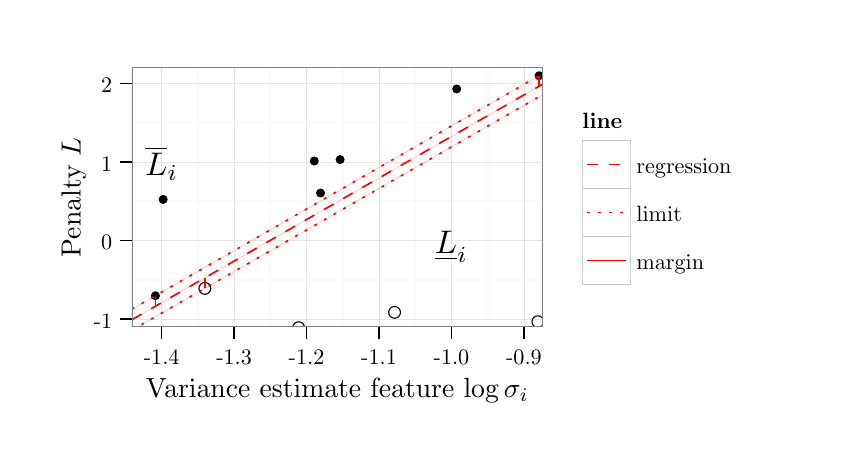
\begin{tikzpicture}[x=1pt,y=1pt]
\definecolor[named]{fillColor}{rgb}{1.00,1.00,1.00}
\path[use as bounding box,fill=fillColor,fill opacity=0.00] (0,0) rectangle (289.08,144.54);
\begin{scope}
\path[clip] (  0.00,  0.00) rectangle (289.08,144.54);
\definecolor[named]{drawColor}{rgb}{1.00,1.00,1.00}
\definecolor[named]{fillColor}{rgb}{1.00,1.00,1.00}

\path[draw=drawColor,line width= 0.6pt,line join=round,line cap=round,fill=fillColor] (  0.00,  0.00) rectangle (289.08,144.54);
\end{scope}
\begin{scope}
\path[clip] ( 37.66, 36.44) rectangle (186.13,130.09);
\definecolor[named]{fillColor}{rgb}{1.00,1.00,1.00}

\path[fill=fillColor] ( 37.66, 36.44) rectangle (186.13,130.09);
\definecolor[named]{drawColor}{rgb}{0.98,0.98,0.98}

\path[draw=drawColor,line width= 0.6pt,line join=round] ( 37.66, 53.47) --
	(186.13, 53.47);

\path[draw=drawColor,line width= 0.6pt,line join=round] ( 37.66, 81.85) --
	(186.13, 81.85);

\path[draw=drawColor,line width= 0.6pt,line join=round] ( 37.66,110.22) --
	(186.13,110.22);

\path[draw=drawColor,line width= 0.6pt,line join=round] ( 61.50, 36.44) --
	( 61.50,130.09);

\path[draw=drawColor,line width= 0.6pt,line join=round] ( 87.68, 36.44) --
	( 87.68,130.09);

\path[draw=drawColor,line width= 0.6pt,line join=round] (113.87, 36.44) --
	(113.87,130.09);

\path[draw=drawColor,line width= 0.6pt,line join=round] (140.05, 36.44) --
	(140.05,130.09);

\path[draw=drawColor,line width= 0.6pt,line join=round] (166.23, 36.44) --
	(166.23,130.09);
\definecolor[named]{drawColor}{rgb}{0.90,0.90,0.90}

\path[draw=drawColor,line width= 0.2pt,line join=round] ( 37.66, 39.28) --
	(186.13, 39.28);

\path[draw=drawColor,line width= 0.2pt,line join=round] ( 37.66, 67.66) --
	(186.13, 67.66);

\path[draw=drawColor,line width= 0.2pt,line join=round] ( 37.66, 96.03) --
	(186.13, 96.03);

\path[draw=drawColor,line width= 0.2pt,line join=round] ( 37.66,124.41) --
	(186.13,124.41);

\path[draw=drawColor,line width= 0.2pt,line join=round] ( 48.41, 36.44) --
	( 48.41,130.09);

\path[draw=drawColor,line width= 0.2pt,line join=round] ( 74.59, 36.44) --
	( 74.59,130.09);

\path[draw=drawColor,line width= 0.2pt,line join=round] (100.78, 36.44) --
	(100.78,130.09);

\path[draw=drawColor,line width= 0.2pt,line join=round] (126.96, 36.44) --
	(126.96,130.09);

\path[draw=drawColor,line width= 0.2pt,line join=round] (153.14, 36.44) --
	(153.14,130.09);

\path[draw=drawColor,line width= 0.2pt,line join=round] (179.32, 36.44) --
	(179.32,130.09);
\definecolor[named]{drawColor}{rgb}{0.00,0.00,0.00}

\node[text=drawColor,anchor=base,inner sep=0pt, outer sep=0pt, scale=  1.18] at (153.14, 62.78) {$\underline L_i$};

\node[text=drawColor,anchor=base,inner sep=0pt, outer sep=0pt, scale=  1.18] at ( 48.41, 91.15) {$\overline L_i$};

\path[draw=drawColor,line width= 0.4pt,line join=round,line cap=round] ( 64.01, 50.33) circle (  2.13);

\path[draw=drawColor,line width= 0.4pt,line join=round,line cap=round] (184.36, 38.29) circle (  2.13);

\path[draw=drawColor,line width= 0.4pt,line join=round,line cap=round] (153.38,  6.61) circle (  2.13);

\path[draw=drawColor,line width= 0.4pt,line join=round,line cap=round] (186.13, 24.56) circle (  2.13);

\path[draw=drawColor,line width= 0.4pt,line join=round,line cap=round] (132.57, 41.67) circle (  2.13);

\path[draw=drawColor,line width= 0.4pt,line join=round,line cap=round] ( 94.46, 29.21) circle (  2.13);

\path[draw=drawColor,line width= 0.4pt,line join=round,line cap=round] (112.83, 16.84) circle (  2.13);

\path[draw=drawColor,line width= 0.4pt,line join=round,line cap=round] (118.78, 11.51) circle (  2.13);

\path[draw=drawColor,line width= 0.4pt,line join=round,line cap=round] (120.11, 23.68) circle (  2.13);

\path[draw=drawColor,line width= 0.4pt,line join=round,line cap=round] (114.20, 21.12) circle (  2.13);

\path[draw=drawColor,line width= 0.4pt,line join=round,line cap=round] (141.34,  4.11) circle (  2.13);

\path[draw=drawColor,line width= 0.4pt,line join=round,line cap=round] (121.45, -0.45) circle (  2.13);

\path[draw=drawColor,line width= 0.4pt,line join=round,line cap=round] (148.35, -0.62) circle (  2.13);

\path[draw=drawColor,line width= 0.4pt,line join=round,line cap=round] ( 97.91, 36.13) circle (  2.13);

\path[draw=drawColor,line width= 0.4pt,line join=round,line cap=round] (104.19, 30.95) circle (  2.13);

\path[draw=drawColor,line width= 0.4pt,line join=round,line cap=round] ( 79.92, 15.58) circle (  2.13);
\definecolor[named]{fillColor}{rgb}{0.00,0.00,0.00}

\path[draw=drawColor,line width= 0.4pt,line join=round,line cap=round,fill=fillColor] ( 46.16, 47.68) circle (  1.42);

\path[draw=drawColor,line width= 0.4pt,line join=round,line cap=round,fill=fillColor] (112.90, 96.86) circle (  1.42);

\path[draw=drawColor,line width= 0.4pt,line join=round,line cap=round,fill=fillColor] ( 48.95, 82.49) circle (  1.42);

\path[draw=drawColor,line width= 0.4pt,line join=round,line cap=round,fill=fillColor] (184.80,127.17) circle (  1.42);

\path[draw=drawColor,line width= 0.4pt,line join=round,line cap=round,fill=fillColor] (105.83, 84.78) circle (  1.42);

\path[draw=drawColor,line width= 0.4pt,line join=round,line cap=round,fill=fillColor] (103.57, 96.34) circle (  1.42);

\path[draw=drawColor,line width= 0.4pt,line join=round,line cap=round,fill=fillColor] (155.03,122.39) circle (  1.42);
\definecolor[named]{drawColor}{rgb}{1.00,0.00,0.00}
\definecolor[named]{fillColor}{rgb}{1.00,0.00,0.00}

\path[draw=drawColor,line width= 0.6pt,dash pattern=on 4pt off 4pt ,line join=round,fill=fillColor] ( 37.66, 39.02) -- (186.13,124.14);

\path[draw=drawColor,line width= 0.6pt,dash pattern=on 1pt off 3pt ,line join=round,fill=fillColor] ( 37.66, 42.81) -- (186.13,127.93);

\path[draw=drawColor,line width= 0.6pt,dash pattern=on 1pt off 3pt ,line join=round,fill=fillColor] ( 37.66, 35.23) -- (186.13,120.35);

\path[draw=drawColor,line width= 0.6pt,line join=round,fill=fillColor] ( 64.01, 50.33) -- ( 64.01, 54.12);

\path[draw=drawColor,line width= 0.6pt,line join=round,fill=fillColor] ( 46.16, 47.68) -- ( 46.16, 43.89);

\path[draw=drawColor,line width= 0.6pt,line join=round,fill=fillColor] (184.80,127.17) -- (184.80,123.38);
\definecolor[named]{drawColor}{rgb}{0.50,0.50,0.50}

\path[draw=drawColor,line width= 0.6pt,line join=round,line cap=round] ( 37.66, 36.44) rectangle (186.13,130.09);
\end{scope}
\begin{scope}
\path[clip] (  0.00,  0.00) rectangle (289.08,144.54);
\definecolor[named]{drawColor}{rgb}{0.00,0.00,0.00}

\node[text=drawColor,anchor=base east,inner sep=0pt, outer sep=0pt, scale=  0.80] at ( 30.55, 35.98) {-1};

\node[text=drawColor,anchor=base east,inner sep=0pt, outer sep=0pt, scale=  0.80] at ( 30.55, 64.35) {0};

\node[text=drawColor,anchor=base east,inner sep=0pt, outer sep=0pt, scale=  0.80] at ( 30.55, 92.73) {1};

\node[text=drawColor,anchor=base east,inner sep=0pt, outer sep=0pt, scale=  0.80] at ( 30.55,121.10) {2};
\end{scope}
\begin{scope}
\path[clip] (  0.00,  0.00) rectangle (289.08,144.54);
\definecolor[named]{drawColor}{rgb}{0.00,0.00,0.00}

\path[draw=drawColor,line width= 0.6pt,line join=round] ( 33.40, 39.28) --
	( 37.66, 39.28);

\path[draw=drawColor,line width= 0.6pt,line join=round] ( 33.40, 67.66) --
	( 37.66, 67.66);

\path[draw=drawColor,line width= 0.6pt,line join=round] ( 33.40, 96.03) --
	( 37.66, 96.03);

\path[draw=drawColor,line width= 0.6pt,line join=round] ( 33.40,124.41) --
	( 37.66,124.41);
\end{scope}
\begin{scope}
\path[clip] (  0.00,  0.00) rectangle (289.08,144.54);
\definecolor[named]{drawColor}{rgb}{0.00,0.00,0.00}

\path[draw=drawColor,line width= 0.6pt,line join=round] ( 48.41, 32.18) --
	( 48.41, 36.44);

\path[draw=drawColor,line width= 0.6pt,line join=round] ( 74.59, 32.18) --
	( 74.59, 36.44);

\path[draw=drawColor,line width= 0.6pt,line join=round] (100.78, 32.18) --
	(100.78, 36.44);

\path[draw=drawColor,line width= 0.6pt,line join=round] (126.96, 32.18) --
	(126.96, 36.44);

\path[draw=drawColor,line width= 0.6pt,line join=round] (153.14, 32.18) --
	(153.14, 36.44);

\path[draw=drawColor,line width= 0.6pt,line join=round] (179.32, 32.18) --
	(179.32, 36.44);
\end{scope}
\begin{scope}
\path[clip] (  0.00,  0.00) rectangle (289.08,144.54);
\definecolor[named]{drawColor}{rgb}{0.00,0.00,0.00}

\node[text=drawColor,anchor=base,inner sep=0pt, outer sep=0pt, scale=  0.80] at ( 48.41, 22.72) {-1.4};

\node[text=drawColor,anchor=base,inner sep=0pt, outer sep=0pt, scale=  0.80] at ( 74.59, 22.72) {-1.3};

\node[text=drawColor,anchor=base,inner sep=0pt, outer sep=0pt, scale=  0.80] at (100.78, 22.72) {-1.2};

\node[text=drawColor,anchor=base,inner sep=0pt, outer sep=0pt, scale=  0.80] at (126.96, 22.72) {-1.1};

\node[text=drawColor,anchor=base,inner sep=0pt, outer sep=0pt, scale=  0.80] at (153.14, 22.72) {-1.0};

\node[text=drawColor,anchor=base,inner sep=0pt, outer sep=0pt, scale=  0.80] at (179.32, 22.72) {-0.9};
\end{scope}
\begin{scope}
\path[clip] (  0.00,  0.00) rectangle (289.08,144.54);
\definecolor[named]{drawColor}{rgb}{0.00,0.00,0.00}

\node[text=drawColor,anchor=base,inner sep=0pt, outer sep=0pt, scale=  1.00] at (111.90, 10.84) {Variance estimate feature $\log\sigma_i$};
\end{scope}
\begin{scope}
\path[clip] (  0.00,  0.00) rectangle (289.08,144.54);
\definecolor[named]{drawColor}{rgb}{0.00,0.00,0.00}

\node[text=drawColor,rotate= 90.00,anchor=base,inner sep=0pt, outer sep=0pt, scale=  1.00] at ( 19.11, 83.26) {Penalty $L$};
\end{scope}
\begin{scope}
\path[clip] (  0.00,  0.00) rectangle (289.08,144.54);
\definecolor[named]{fillColor}{rgb}{1.00,1.00,1.00}

\path[fill=fillColor] (196.20, 47.50) rectangle (264.55,119.03);
\end{scope}
\begin{scope}
\path[clip] (  0.00,  0.00) rectangle (289.08,144.54);
\definecolor[named]{drawColor}{rgb}{0.00,0.00,0.00}

\node[text=drawColor,anchor=base west,inner sep=0pt, outer sep=0pt, scale=  0.80] at (200.47,108.14) {\bfseries line};
\end{scope}
\begin{scope}
\path[clip] (  0.00,  0.00) rectangle (289.08,144.54);
\definecolor[named]{drawColor}{rgb}{0.80,0.80,0.80}
\definecolor[named]{fillColor}{rgb}{1.00,1.00,1.00}

\path[draw=drawColor,line width= 0.6pt,line join=round,line cap=round,fill=fillColor] (200.47, 86.46) rectangle (217.81,103.80);
\end{scope}
\begin{scope}
\path[clip] (  0.00,  0.00) rectangle (289.08,144.54);
\definecolor[named]{drawColor}{rgb}{1.00,0.00,0.00}

\path[draw=drawColor,line width= 0.6pt,dash pattern=on 4pt off 4pt ,line join=round] (202.20, 95.13) -- (216.08, 95.13);
\end{scope}
\begin{scope}
\path[clip] (  0.00,  0.00) rectangle (289.08,144.54);
\definecolor[named]{drawColor}{rgb}{0.80,0.80,0.80}
\definecolor[named]{fillColor}{rgb}{1.00,1.00,1.00}

\path[draw=drawColor,line width= 0.6pt,line join=round,line cap=round,fill=fillColor] (200.47, 69.11) rectangle (217.81, 86.46);
\end{scope}
\begin{scope}
\path[clip] (  0.00,  0.00) rectangle (289.08,144.54);
\definecolor[named]{drawColor}{rgb}{1.00,0.00,0.00}

\path[draw=drawColor,line width= 0.6pt,dash pattern=on 1pt off 3pt ,line join=round] (202.20, 77.78) -- (216.08, 77.78);
\end{scope}
\begin{scope}
\path[clip] (  0.00,  0.00) rectangle (289.08,144.54);
\definecolor[named]{drawColor}{rgb}{0.80,0.80,0.80}
\definecolor[named]{fillColor}{rgb}{1.00,1.00,1.00}

\path[draw=drawColor,line width= 0.6pt,line join=round,line cap=round,fill=fillColor] (200.47, 51.77) rectangle (217.81, 69.11);
\end{scope}
\begin{scope}
\path[clip] (  0.00,  0.00) rectangle (289.08,144.54);
\definecolor[named]{drawColor}{rgb}{1.00,0.00,0.00}

\path[draw=drawColor,line width= 0.6pt,line join=round] (202.20, 60.44) -- (216.08, 60.44);
\end{scope}
\begin{scope}
\path[clip] (  0.00,  0.00) rectangle (289.08,144.54);
\definecolor[named]{drawColor}{rgb}{0.00,0.00,0.00}

\node[text=drawColor,anchor=base west,inner sep=0pt, outer sep=0pt, scale=  0.80] at (219.98, 91.82) {regression};
\end{scope}
\begin{scope}
\path[clip] (  0.00,  0.00) rectangle (289.08,144.54);
\definecolor[named]{drawColor}{rgb}{0.00,0.00,0.00}

\node[text=drawColor,anchor=base west,inner sep=0pt, outer sep=0pt, scale=  0.80] at (219.98, 74.48) {limit};
\end{scope}
\begin{scope}
\path[clip] (  0.00,  0.00) rectangle (289.08,144.54);
\definecolor[named]{drawColor}{rgb}{0.00,0.00,0.00}

\node[text=drawColor,anchor=base west,inner sep=0pt, outer sep=0pt, scale=  0.80] at (219.98, 57.13) {margin};
\end{scope}
\end{tikzpicture}
